\section{Multi-band Adaptation Model}
\label{sec:model}
%fixme: why did you use this model versus another?  you have not explained all the terms (d_0) or related the terms to the description (\lambda, PL).
In this section, we introduce the path-loss relationship across frequency bands and explain the theoretical gains a multi-band adaptation protocol could expect to achieve. Path loss increases with distance from the base and related to the wavelength the decibel path loss can be presented as:\cite{rappaport}

\begin{equation}
P_{R}=\frac{P_TG_TG_R\lambda}{d^\alpha(4\pi)^2}
\end{equation}

where ,$P_R$ is the received signal of receiver node, $P_T$ is the transmitting power, $G_T,G_R$ represent the antennas gain at both transmitting and receive nodes,
$\lambda$ is the wavelength, $\alpha$ is the path loss exponent related to the environment. 

%In an ideal channel, if the received signal is the same among all the bands, the performance should be the same. It is a reasonable assumption verified by experiments on the emulator. The performance across different bands in different received signal shows as: {fixme insert throughput vs rssi in bypass}
We focus on a point to point communication pair system. 
From the equation, the attennas gain $G_T,G_R$ is fixed for a communication system, and the distance from the transmitter to the receiver is fixed.
And also due to limitations imposed by the FCC, the transmit power $P_T$ of an access point is restricted. 
So in such a wireless system, the $P_R$ of the receive node is determined by two parameters. One is the path loss exponent $\alpha$, another is the wavelength of the operating channel. 
Our research focus on the situation the radios in different bands work on the same node, they operate in the same environment, so the path loss exponent for different bands should be the same. 
The path loss exponent in an evnironment usually be estimated by measuring the received power and distance between the transmit and receive nodes. According to these measurements, a fitting exponent curve can be used to get the path loss exponent. fixme insert rx-power and distance graph 

Then, for a multi-band/multi-radio system can work on different bands, wavelength become the most important factor influence the received power.
In an ideal channel, if the received signal is the same among all the bands, the performance should be the same. It is a reasonable assumption verified by experiments on the channel emulator. The performance across different bands in different received signal shows as: {fixme insert throughput vs rssi in bypass}

%In the limited access range, the path loss of different bands are varying according to their wavelength. 
The difference of received signal makes the performance vary in different bands. Then, for a particular environment, there is room to improve the performance in switching band.


Another potential room  for wireless communication performance improvement is the utility level of a channel. Most of the wifi devices are working in 2.4GHz and 5GHz as 802.11 standard. Other interference signals, such as TV, GSM signals are shown in other bands. These interference signals, both 802.11 signals and other interference signals, are discontinuous. 
For a multi-band communication, we treat these signals as primary users, try to find the spectrum opportunity and imprvoe the performance.

%Our method is to employ accumulate information in a time slot to quantify the channel state. The difference in crowd level of wireless channel also provide room for performance improvement in switching band.  
%In this section, we exploit channel dynamic and accumulate information in contextual data and develop band adaptation frame for dynamic environments.Through the proposed framework, we improve the throughput of a pair of multi-radio nodes according the given context. While in this paper we focus on the application to band adaptation to show gains, the framwork has other possible applications to transmission parameter adaptation based on context information. 


\subsection{Problem Formulation}
\label{subsec:problem}
%room for improvement
Spectrum sensing is the fundamental problem of cognitive radio and has reborn as a very active research area in recent years despite its long history\cite{zeng2010review}.
%It can be classed as \emph{Energy Detector Based Sensing, Matched Filter Detection, Cyclostationary Detection, Wavelet-based Detection, etc.} \cite{zeng2010review,zhao2007survey}.


%Objective
The objective of this work is to improve the performance of multi-bands system in pratical environments based on limited information of a communication system.
It is also very important for our framework to detect the channel state.
%previous research no propagation, no map to throughput
Most of the previous research of spectrum sensing focus on the theoretical computation of detection probability and false alarm probability without considering the difference of propagation across different bands \cite{zeng2010review,zhao2007survey,chen2008joint,hou2011spectrum}. 
In pratice, there are other factors such as system loss which could not be theoretical analyzing make it hard to exploit these spectrum sensing algorithms.
Moreover, these researches do not show any wireless performance information related to the spectrum sensing directly. 

%Protocol has been built

There are multi-channel adaptation and rate adaptation researches focus on \emph{Dynamic Channel State} as represented by \cite{cordeiro2007c,MOAR}:. 

\begin{equation}
f(SNR,Context-Aware\, Info) \rightarrow Performance Estimation
\end{equation}

which distinguish that the performance is related to the channel state, but only involve the dynamic information. 
However, the embedded temporal correlation of the wireless channel also represent the channel state \cite{liuastra}. 
%The interference factor gradually changing process makes the statistics have an embedded temporal correlation. 


%This paper's work
The context-aware information provide a way to resolve the problem. History information can be exploited for spectrum sensing prediction \cite{yucek2009survey}.
Our work involve the historical information in an environment to do the spectrum sensing considering the difference of propagation across wifi bands and non-wifi bands. 
A performance mapping from the spectrum sensing is introduced and evaluated by experiments.



In this framework,there are several steps to approach the objective. 
First step is to do the spectrum sensing and gather information across different bands. 
Second is to predict performance among all the bands based on the spectrum sensing information. 
Furthermore, we adjust the estimation according to the \emph{Activity Level} present the utility level of the channel.
Then, switching decision is made after all these steps.



%The performance context-aware database is created on simulated channel. The input of the database includes channel type, velocity and SNR.
%Channel type indicates the propagation and fading characteristics between the transmitter and receiver. Many factors(e.g., multi-path, path loss, and shadowing) have a substantial influence on the characteristics of the channel type \cite{liuastra}. We use ITU channel types to generate the performance database, which are widely accepted as representative channel types for urban and suburban settings \cite{recommendation19971225}.


%The objective of this work is to demonstrate the improvements in performance by leveraging information of ideal channels to make band adapatation decisions. As noted before, the context information we consider is the channel type, measured received signal strength, received bytes, background noise and channel interference. The channel type indicates the propagation and fading characteristics between the transmitter and receiver. Many factors(e.g., multi-path, path loss, and shadowing) have a substantial influence on the characteristics of the channel type.FIXME{citation of Hui paper} However, in this paper, we assume the channel type to be a static channel type across all the wireless bands. We use the defination of ITU channels, which are widely accepted as representative channel types for urban dan suburban settings \cite{recommendation19971225}. Moreover, noise and interference gradually changes in the field. The gradually changing process makes it possible to seperate the noise, and even the interference from time varying experiments. 

%As far as we know, there is no work has done for such multi-band adaptation. 

%Problem formulation, equation style
The optimization problem can be formulated as: in multi-radio/multi-bands system, given dynamic received signal level in part of the available bands, the activity level of all the bands, and context-aware information, which spectrum band should we choose. 




%We adapt the transmission band for each scenario based on the contextual information and the temporal correlation. 

%In this paper, we involve a factor \emph{Activity Level} to the framework. In this case, the multi-band adaptation can be simply represented as:

\begin{equation}
f(Part\, Bands\, Signal\, Level, All\,bands\, Activity\, Level,Context-Aware\, Info)\\
\rightarrow max_{One Band}{Performance Estimation}
\end{equation}

The \emph{Activity \, Level} is defined as a statistics of band occupied time ratio. Through the temporal correlation parameter, the prediction of the performance could fits in-field system channel state estimation better than only consider the dynamic channel state.


%fixme, the figure should include the rssi estimate
\begin{figure}
\centering
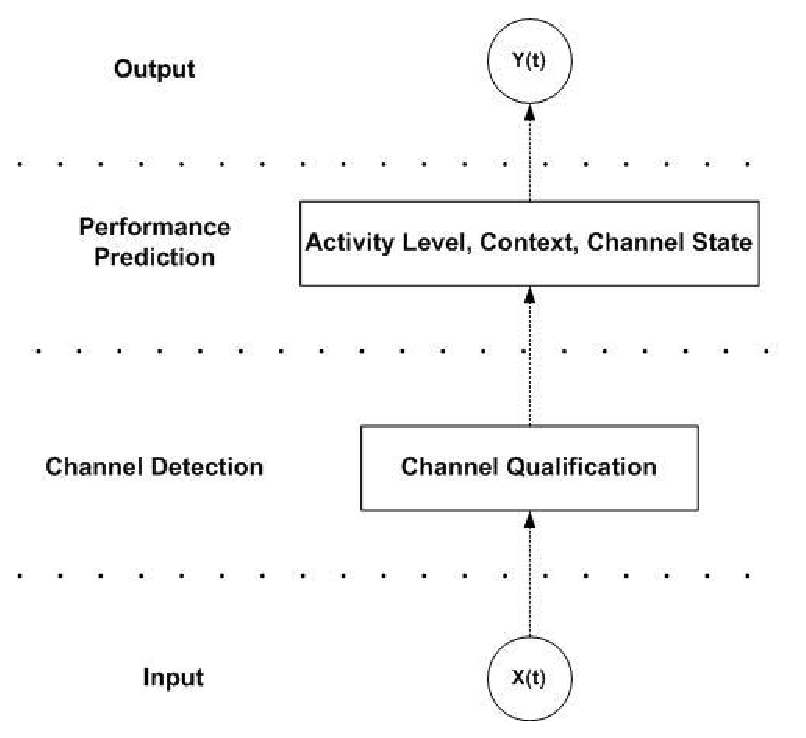
\includegraphics[width=85mm]{figure/multiband_framework}
\caption{Multi-band framework.}
\label{fig:multiframe}
\end{figure}




\subsection{Performance Prediction and Decision}

The multi-band adaptation is receiver driven: the receiver node estimate the channel state, computes the optimal choice of band across all the band, and feeds it back to the sender. 
The process of estimation is described as follows.

Let set $S$ denote the n-tuple of the number of bands can be selected. In the numerical results, we consider the set $S$ for white space and current common wifi wireless bands. $S={m}$, where $m \in \{\mbox{\it 450MHz},\mbox{\it 2.4GHz},\mbox{\it 5.8GHz}\}$ represents the band that is selected. 
Let C represent the possible context information from previous measurements for a particular band with given parameters.

In this paper, the optimization metric of interest is the measured throughput $t_put$. 
%The optimization problem is stated as follows: 
Given a particular context ${c\in C}$, select the optimal $s^* \in S$ that maximizes the throughput, $G_{th}$ 
Formally, the problem is posed as follows:


\begin{eqnarray}
\max_{s \in S}& G_{th}& = (1-\mbox{\it Activity Level})*R_{th} \label{eq:throughput_optimization} \\
		\mbox{\it given} & & \mbox{\it Signal Strength}, \mbox{\it velocity}, \mbox{\it channel type} \nonumber
		\end{eqnarray}

$T_{ideal}$ is the throughput from the ideal channel conditions in emulator. 
%where Activity Level is a ratio as notified represent the time during one period occupied by other nodes. 

%The optimization problem is solved through several steps in our framework with the context-aware information.

%-up table has the relationship of SNR and throughput mapping generated from experiments in ideal channel states, in our case collecting the data on channel emulator.  



\begin{align}
&w_{k}(t+1) = w_{k}(t) + \tau_{k}(\alpha_{k}(1 - w_{k}(t))\nonumber \\
&~~~~~~~~- w_{k}(t)x(t)),~~(0<k\le{n})
\label{eq:habituation}
\end{align}


\subsection{Context-Aware Information}

%1,what is context info


Contexts, which defines various operating situations. Depending on a context, the wireless device changes its operational 
behavior in accordance with a defined profile, when a context parameter changes \cite{phillips2004wireless}. Context is a database include the knowledge the system stored or learned from the experiments or activities. Based on tons of measurement in different scenarios, a relationship between performance and system parameters can be created. 
For each piece of input parameters, the database can provide an output according to different algorithms.
%The collected contextual information is the input to the multi-band adaptaion model. In the ideal channel context information, for each given set of bands, SNR, the context table can represent ideal throughput for each bands. 

%2,how others use the info Fixme
In wireless communication, context-aware information is the experience of a transmit receiver pair. The performance of a system in the past can help transmute to find the optimal rate/band based on the parameter collected by the receiver. Such as in FARA algorithm, the receiver uses an SNR characterization table that lists the minimum SNR required for a particular combination of modulation and coding rate\cite{rahul2009frequency}. 
%3,how we use the info

In this paper, two context-aware database are exploited, one is the context-aware database for signal level across different bands, another one is the performance database. 
In the signal level context database, the input is signal level of one band, the output includes the signal level of other bands.
In the performance context information, we input the signal level, velocity and channel type to the database, then output the estimated throughput.  
%4,Difference
The output throughput is the middle state of our model to get the prediction of the performance, furthermore, adjustment will be put on these information. 


\begin{equation}
f(Part\, Band\, Signal\, Level) \rightarrow Multi-band Signal Level
\end{equation}

\begin{equation}
f(Signal\, Level,Channel\, Type, Velocity, \\ 
Context-Aware\, Info) \rightarrow Performance Estimation
\end{equation}




\subsection{Dynamic and Correlation Info}

%1,How to evaluate channel
Signal level is widely used to represent the dynamic channel state  \cite{rahul2009frequency}. 
%2,SNR
Many hardware manufactures already perform the SNR/Received signal strength detection character as part of the hardware specification \cite{edalat2006measured}. 
Mapping the signal level value to the context information is widely used in cognitive radio for estimation \cite{laneman2000energy,laneman2001efficient}. 

%In this paper, signal level is also an important factor for the performance database.
%3,Loss based
Otherwise, the factors except signal level also has information about the channel state. Statistics information is used by lots of adaptation algorithms.
FARA tracks the the number of active clients, then update the next-hop table for transmission\cite{rahul2009frequency}.
The statistics of collisions and link errors also could be considered as channel qualification factors \cite{pang2005rate}.
The activity level present the utility level of wireless channel is defined as a factor of the channel accumulate in time domain to estimate the wireless performance.
%4,The definitation of the activity level
In our work, the definition of activity can be represented by:

%Non 802.11 interference
For the white band whose first user is TV or cellphones, the activity level is defined as:
\begin{equation}
\label{equation:non802 Activity Level}
Activity\,Level = \sum{\frac{Interference Active Time}{Duration}}
\end{equation}
%802.11 interference
For 802.11 standard band, 2.4GHz and 5GHz, the activity level is defined as:
\begin{equation}
\label{equation:802 Activity Level}
Activity\,Level = \sum{\frac{(Total\, Packets)-(Connection\, Packets)}{Rate*Duration}}
\end{equation}

Total packets is the amount of packets received in one band during a time slot.
The connection packets is the amount of packets received by particular transmitter and receiver pair. 
The length and transmitting rate of each packet are collected to calculate the activity level.
The \emph{Activity Level} is a \emph{ratio} that occupied by the interference transmitter during a time slot. 
%We assume all the nodes have a common rate or could be averaged to a transmission rate. 
It represents the free time ratio can be used by the particular transmitter and receiver transmission. 
The transmission of interference nodes has correlation between continuous periods, especially the beacon packets. So the previous channel state can be used as a parameter for estimating current channel states.

%5,How we use these information
%Fixme{Figure}


Different variations of \ref{eq:throughput_optimization} we consider include: 
(\emph{i}) We map the context-aware information to find the maximize throughput across the bands in vehicular channel model.
(\emph{ii}) We verify our protocol through in-field experiments data collecting on campus in vehicles. 
The corresponding maximal throughput,$G^*$, serves as an upper bound to the performance that can be achieved by multi-band adaptation. 
This upper bound is computed from the training data on emulator employing SVM as the performance in ideal channel and all transmission time is free to use for the focused transmission pair.



To be clear, we list the steps of the framework for multi-band as follow:

\begin{itemize}
\item \emph{Step 1} Create the signal level database for a location. The connection across different bands can be distinguished in this context-aware database.
%\item \emph{Step 1} Collect context data on emulator for different scenarios (Bands, Channel type, SNR, Velocity) to find the ideal state or the upper bound of the performance for one band.
\item \emph{Step 2} Collect context data on emulator for different scenarios (Bands, Channel type, SNR, Velocity) to create the performance database for the ideal state or the upper bound of the performance for each band.
\item \emph{Step 3} Detect the signal level in one band to qualify the wireless channel in all the bands dynamically, map the estimate signal level to the performance context-aware information in \emph{Step 2} finding the upper bound of for the current wireless channel state.  
\item \emph{Step 4} Compute the \emph{Activity Level} according to the statistic information, then re-calculate the estimate throughput including the \emph{Activity Level}.
\item \emph{Step 4} Compare the estimate throughput across all the bands and make the best choice among the available bands.
\end{itemize}

Through these steps, the transmitter and receiver pair updates the channel state and put the best band in working.





		%Fixme



